% 제7회 한국 인공지능 학술대회 (KICS 인공지능소사이어티) 투고 원고
% 조판 수치 출처: 학회 한글 양식(양식-논문샘플한글.hwp) — 여백 1.5cm(머리말 1.0cm 포함 상단 2.5cm),
%   단 간격 0.5cm, 본문 9pt·장평 90%·자간 -7%(영문 -5%), 제목 13pt·저자 11pt·요약 9pt.
%   줄간격은 워드 양식(1줄)에 맞춘 11pt.
\documentclass[a4paper,twocolumn,9pt]{extarticle}
\usepackage{kotex}
\setmainfont[FakeStretch=0.9,LetterSpace=-5]{lmroman10-regular.otf}[BoldFont=lmroman10-bold.otf,ItalicFont=lmroman10-italic.otf]
\setmainhangulfont[FakeStretch=0.9,LetterSpace=-7]{UnBatang.ttf}[BoldFont=UnBatangBold.ttf]
\usepackage[left=1.5cm,right=1.5cm,top=2.5cm,bottom=1.5cm]{geometry}
\usepackage{graphicx}
\usepackage{amsmath}
\usepackage{setspace}
\usepackage[font=small,skip=3pt]{caption}
\usepackage{xcolor}
\usepackage[hidelinks]{hyperref}   % 인용·그림 번호 클릭 시 해당 위치로 점프

\setlength{\columnsep}{0.5cm}
\pagestyle{empty}


\renewcommand{\thesection}{\Roman{section}.}
\makeatletter
\renewcommand\section{\@startsection{section}{1}{\z@}%
  {1.2ex plus .5ex}{0.8ex plus .3ex}{\normalsize\bfseries}}
\makeatother

\begin{document}


\twocolumn[{
\begin{center}\addfontfeatures{FakeStretch=1,LetterSpace=0}\addhangulfontfeatures{FakeStretch=1,LetterSpace=0}
{\large\bfseries VLA 모델이 스스로 인지하는 작업 단계의 실시간 감지}\\[1.2ex]
{박경태, 김상우, 오윤선$^{\dagger}$}\\
{한양대학교}\\[0.6ex] 
{\small rudxo1997@hanyang.ac.kr, kimz1121@hanyang.ac.kr, $^{\dagger}$yoh21@hanyang.ac.kr}\\[2.0ex] 
{\large\bfseries Real-Time Detection of a VLA Model's Self-Perceived Action Phase}\\[1.2ex]
{Kyungtae Park, Sangwoo Kim, Yoonseon Oh$^{\dagger}$}\\ 
{Hanyang University}\\[2.0ex]
{\bfseries 요 약}\\[0.8ex]
\end{center}
\begin{quote}\small
Vision-Language-Action(VLA) 모델이 작업을 수행할 때 스스로 현재 어떤 작업 단계(action phase)를 진행 중인지를 우리가 알 수 있다면, 이는 VLA 모델에 대한 설명 가능성을 높이고 추론 중 제어 및 개입을 가능하게 하는 출발점이 된다. 본 연구는 모델이 현재 수행 중인 action phase를 model의 내부 activation에서 감지할 수 있음을 보인다. GR00T N1.5 모델의 action head(diffusion transformer, DiT)의 residual stream activation을 clustering하면, 각 cluster는 특정 action phase에 국한되어 나타나고 다른 phase에서는 잘 나타나지 않는다. 이 대응을 이용하면 학습에 사용하지 않은 unseen scene에서도 한 step의 activation만으로 현재 phase를 0.82의 정확도로 감지할 수 있으며, 이는 경과 시간을 등분위로 분할하여 만든 시간 대조군과 관찰 기반 외부 모델 대조군을 웃돈다. 이 구조는 압축 모델을 SAE로 바꾸어 실험해도 재현된다. 즉 VLA activation에는 phase와 정합적인 구조가 존재해 이를 통해 추론 중 online action phase detection이 가능하다.
\end{quote}
\vspace{0.3ex}
}]

\begin{figure}[!t]
  \centering
  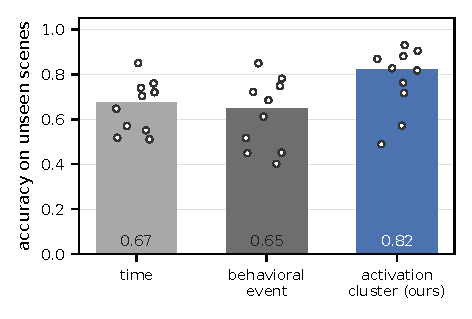
\includegraphics[width=0.86\columnwidth]{figs/fig_readout_bar.pdf}
  \caption{Unseen scene에서의 phase 감지 정확도. 막대는 instruction 10개의 중앙값, 흰 점은 instruction 별 값이다. 회색은 외부 정보만 쓰는 대조군, 파랑은 내부 activation이다.}
  \label{fig:readout}
\end{figure}
\section{서 론}
VLA 모델은 내부를 이해하기 힘든 블랙박스이지만 실제 로봇을 조작하므로, 모델이 지금 무슨 작업을 진행 중이라고 인지하는지 사람이 파악할 수 있어야 한다. 본 논문에서 action phase란 manipulation task를 의미 단위로 나누었을 때 로봇이 수행하고 있는 하위 작업(subtask)을 의미한다. 같은 subtask가 한 task 안에서 여러 번 다시 등장할 수도 있다. 예컨대 Pick \& Place task는 reach, grasp, transport, place의 phase로 구성된다\cite{options}. 현재 phase를 파악하는 방법으로는 카메라나 센서로 얻은 환경, 로봇의 상태정보를 통해 외부 관찰자 모델을 학습시켜서 얻는 방법이 있다\cite{lotus}. 하지만 외부 관찰은 로봇이 겉보기에 무엇을 하는지 알려줄 뿐이며, 모델이 스스로 어떤 작업을 하고 있다고 인지하는지는 내부 activation을 직접 읽어야만 알 수 있고, 이는 겉보기 행동과 모델의 인지가 어긋났을 때 수정을 위한 전제 조건이다. VLA 내부 표현을 해석하려는 최근 시도들은 Sparse Auto Encoder(SAE)나 linear probe로 primitive action에 대응하는 feature를 찾고 그 방향으로 steering까지 보였으나\cite{saevla,observing,egsae,mechinterp}, feature의 이름은 사람이 rollout 영상과 대조해 수동으로 붙이며, 내부 표상이 사람이 정의한 phase를 얼마나 정확히, 어떤 단위로 담는지는 정량화하지 않는다. VLA의 내부 phase를 추론 중에 online으로 읽을 수 있으면 설명을 넘어 조건부 개입이나 실패 감지\cite{safe}의 조건 신호로 활용할 수 있다. 본 연구는 GR00T N1.5\cite{groot}가 RoboCasa\cite{robocasa} 주방 조작을 수행하는 동안의 activation을 Auto Encoder(AE)와 clustering으로 분석해, 모델 내부 phase가 사람이 정의한 phase와 갖는 관계를 감지 정확도와 Mutual Information(MI) margin으로 정량화한다.

\section{방 법}
\textbf{Data.} RoboCasa 주방 조작 환경에서 GR00T N1.5의 rollout을 수집한다. 5개 task(OpenDrawer, PnPCounterToCab, OvenRack, DishwasherRack, CoffeeSetupMug)에 속하는 10개 instruction마다 10개 scene에서 10회씩 총 1{,}000 rollout을 수집하였다. 모델이 1회 추론할 때마다 action head(DiT)의 residual stream activation을 캡처하며, 이 추론 1회를 한 추론 스텝으로 삼는다. 이 activation은 12번째 layer의 마지막 denoising step에서 49개 토큰을 평균한 1{,}536차원 벡터이고, GT phase 라벨은 그 추론이 일어난 시점의 라벨을 사용한다.

Detector의 학습과 평가는 instruction별로 진행하며 dataset은 scene 단위로 분리한다. 10개 scene 중 8개를 학습용, 2개를 평가용으로 나누고, 이러한 분할을 무작위로 3가지 구성한다. 분할마다 표준화, AE, clustering, phase 매핑을 학습 scene만으로 새로 fitting하며, 세 분할의 평가 결과를 평균해 보고한다. 사람이 라벨링한 phase 라벨은 AE와 KMeans 학습에는 쓰지 않으며, cluster를 최빈 phase에 대응시키는 매핑과 평가 시 채점에만 사용한다.

\textbf{Clustering.} Raw activation 1{,}536차원을 AE를 통해 16차원 latent 벡터로 압축한 뒤 KMeans로 clustering한다. Cluster 수는 $k=8$을 사용한다. 사람이 라벨링한 phase 수(3--6)를 넘는 $k$에서 감지 성능이 평탄화 돼 특정 $k$에 의존적이지 않음은 결과에서 보인다(Figure~\ref{fig:ksweep}). Cluster 중심은 학습 split에서만 만든다. 추론 중에는 매 추론 스텝마다 얻는 activation을, 학습한 AE에 그대로 통과시켜 latent 값을 얻고 가장 가까운 중심에 배정해 cluster를 추정한다. 이 방식은 추론 중 학습이나 clustering이 필요 없고, 해당 스텝의 activation 하나와 고정된 중심만으로 감지하여 과거·미래 스텝을 필요로 하지 않으므로 online detection이 가능하다.

\textbf{Baseline.} 각 instruction 별로 phase는 순서대로 진행되는 경향이 있다. 따라서 activation이 아니라 단순히 진행도만으로 판단하는 detector도 어느 정도 phase를 맞힌다. 이 몫을 빼기 위한 \textbf{시간 대조군}은 에피소드 시작부터의 경과 스텝 수를 발견된 cluster 수와 같은 개수의 구간으로 등분위 분할한 후, 각 구간별로 학습 데이터에서의 최빈값을 phase로 판단하는 baseline이다. 또한 외부 관찰만으로 phase를 나누는 기존 방법과 비교하기 위해, \textbf{관찰 기반 외부 모델 대조군}으로 기존 연구\cite{egsae}의 이벤트 발견 파이프라인을 채택한다. 저자가 공개한 구현을 수정 없이 사용하여, end-effector 궤적에서 AWE\cite{awe}로 waypoint를 추출하고 그 주변 프레임의 SigLIP\cite{siglip} 시각 임베딩에 로봇 상태와 진행도를 이어붙인 descriptor를 clustering해 이벤트를 얻는다.

\textbf{Metric.} 주 지표는 margin과 정확도이다. 스텝 $i$의 cluster 라벨을 $z_i \in \{1,\dots,k\}$, 사람이 붙인 GT phase를 $y_i$라 하자. Cluster 라벨을 알았을 때 phase에 대한 불확실성이 얼마나 줄어드는지를 Mutual Information(MI)
\begin{equation*}
I(Z;Y)=\sum_{k}\sum_{c} p(k,c)\log_2\frac{p(k,c)}{p(k)p(c)}
\end{equation*}
로 측정한다. 여기서 $p(k,c)$는 전체 스텝 중 cluster가 $k$이면서 phase가 $c$인 비율이다. 다만 MI는 cluster 수가 늘면 자동으로 커지므로, 같은 상태 수를 갖는 시간 대조군의 MI를 뺀 값을 사용한다.
\begin{equation}
\mathrm{margin} = I(Z;Y) - I(Z_{\mathrm{clock}};Y).
\label{eq:margin}
\end{equation}
정확도는 감지한 cluster가 매핑된 phase와 GT phase가 일치하는 비율로 구한다.

\begin{figure*}[!t]
  \centering
  
\includegraphics[width=0.64\textwidth]{figs/fig1_purity_residual.pdf}
  \caption{(a) Cluster와 GT phase 출현 연관성 행렬. 세로축은 cluster에 임의로 부여한 index이다. 이는 특정 cluster는 특정 phase에 주로 국한되어 나타냄을 보여준다. (b) Activation에서 scene별 평균값을 뺀 후의 phase에 대한 margin. (c) activation이 scene에 대해서 얼마나 설명하는지를 나타내는 그래프.}
  \label{fig:purity}
\end{figure*}
\section{결 과}
\textbf{VLA 내부 activation 한 스텝만으로 phase를 감지 할 수 있다.} Instruction별 unseen scene 정확도의 중앙값은 0.82이다(Figure~\ref{fig:readout}). 시간 대조군은 정확도 0.67이며, 관찰 기반 외부 모델 대조군\cite{egsae}은 0.65이다. 같은 환경에서 activation cluster(ours)는 10개 instruction 중 9개에서 관찰 기반 외부 모델 대조군을 앞서며, 모든 방법이 약 0.5의 정확도를 보이는 ``Fully slide the top dishwasher rack out'' instruction에서는 예외이다. 즉 내부 activation이 가진 phase 정보가 가장 풍부하고 정확하다.

\textbf{각 cluster는 특정 phase에 국한된다.} 한 phase에서 나타난 cluster는 다른 phase에서 잘 나타나지 않는다. Cluster와 phase의 동시 출현 비율 $p(k,c)$를 나타낸 행렬에서는 특정 cluster는 특정 phase에 주로 나타남이 보인다(Figure 2a). 시간 대조군의 MI 중앙값은 0.279 bits이며, margin의 중앙값은 +0.343 bits이다. 모든 instruction에서 양수이므로 단순히 진행도만 가지고 판단하는 것보다 정보량이 풍부함을 알 수 있다(Figure 2b). $k$가 GT phase 수보다 커서 한 phase를 여러 cluster가 나눠 갖더라도 각 cluster는 특정 phase에 국한되므로 이 방식의 높은 정보량을 여전히 지지한다.

\begin{figure}[!t]
  \centering
  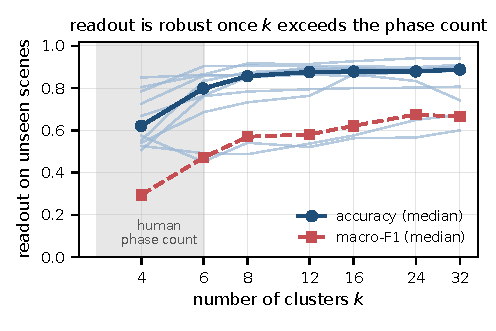
\includegraphics[width=0.86\columnwidth]{figs/fig_k_sweep.pdf}
  \caption{감지 정확도의 $k$에 대한 강건성. GT phase 수(3--6, 회색 대역)를 넘는 $k\ge8$에서 성능이 평탄해진다(0.82--0.88). 흐린 선은 각 instruction별 accuracy 그래프이다.}
  \label{fig:ksweep}
\end{figure}
\textbf{Phase 정보는 장면 암기로 환원되지 않는다.} Activation에는 scene 정보도 섞여 있다(instruction별 scene과의 MI 0.02$\sim$0.86 bits). 그러나 scene별 평균을 제거한 잔차에서 scene 정보는 중앙값 0.44에서 0.27 bits로 크게 줄어드는 반면, phase margin +0.34에서 +0.31로 10개 instruction 전부에서 양수로 유지된다(Figure 2b).

\textbf{Cluster 전환은 압축 모델에 관계없이 일관된다.} Cluster 전환이 특정 압축 모델의 산물이 아님을 확인하기 위해, 같은 activation을 AE와 SAE로 각각 압축·clustering했다. 각 모델은 에피소드의 스텝마다 cluster를 하나씩 배정하므로 앞 step과 cluster가 달라지는 지점을 전환으로 정의할 수 있다. 두 모델이 낸 전환을 $\pm$1스텝 이내에서 짝지었다. 짝지어진 비율을 AE 전환 기준(precision)과 SAE 전환 기준(recall)으로 구해 조화평균한 값이 전환 일치 F1이며, 전환 개수는 두고 위치만 무작위로 흩은 상태열 300개의 F1 분포로 z를 구한다. 두 모델의 전환 일치율은 F1 0.66$\sim$0.75, z +8.8$\sim$+13.5을 보인다. 즉 activation에는 전환 시점 정보가 존재한다.

\section{한계와 결론}
\textbf{한계.} 평가는 단일 모델(GR00T N1.5)·단일 벤치마크(RoboCasa, 시뮬레이션)에 한정되어 다른 VLA나 실제 로봇으로의 일반화는 확인하지 않았다. GT phase 라벨은 한 명의 연구자가 부여한 것이라 정확도의 절대값은 그 기준에 의존한다. 다만 모든 방법을 같은 라벨로 채점하므로 비교에는 영향이 같다. 또한 본 연구는 표상을 읽는 것이며, 개입해 행동을 바꾸는 것은 별개의 검증을 요한다.

\textbf{결론.} VLA의 action head activation에는 사람이 정의한 phase와 정합적인 구조가 있음을 비지도 clustering으로 확인 할 수 있으며, 이를 이용하면 unseen scene에서도 한 스텝의 activation만으로 현재 phase를 정확도 0.82로 감지할 수 있다. 이 감지는 추론 중 매 스텝 online으로 그대로 수행되므로, phase 조건부 개입·실패 감지의 조건 신호로 나아가는 출발점이 된다.

\renewcommand{\refname}{\centering 참 고 문 헌}
\begin{thebibliography}{99}\scriptsize\setlength{\itemsep}{0pt}\setlength{\parskip}{0pt}
\bibitem{groot} NVIDIA GEAR Team, ``GR00T N1: An Open Foundation Model for
Generalist Humanoid Robots,'' arXiv:2503.14734, 2025.
\bibitem{robocasa} S. Nasiriany et al., ``RoboCasa: Large-Scale Simulation of
Everyday Tasks for Generalist Robots,'' \textit{RSS}, 2024.
\bibitem{saevla} A. Swann et al., ``Sparse Autoencoders Reveal Interpretable and
Steerable Features in VLA Models,'' arXiv:2603.19183, 2026.
\bibitem{observing} H. Buurmeijer et al., ``Observing and Controlling Features in
Vision-Language-Action Models,'' arXiv:2603.05487, 2026.
\bibitem{egsae} X. Jin et al., ``Event-Grounded Sparse Autoencoders for
Vision-Language-Action Policies,'' arXiv:2605.17204, 2026.
\bibitem{awe} L. X. Shi, A. Sharma, T. Z. Zhao, and C. Finn, ``Waypoint-Based
Imitation Learning for Robotic Manipulation,'' \textit{CoRL}, 2023.
\bibitem{siglip} X. Zhai, B. Mustafa, A. Kolesnikov, and L. Beyer, ``Sigmoid Loss
for Language Image Pre-Training,'' \textit{ICCV}, 2023.
\bibitem{mechinterp} B. H\"aon et al., ``Mechanistic Interpretability for Steering
Vision-Language-Action Models,'' \textit{CoRL}, 2025.
\bibitem{safe} Q. Gu et al., ``SAFE: Multitask Failure Detection for
Vision-Language-Action Models,'' \textit{NeurIPS}, 2025.
\bibitem{lotus} W. Wan et al., ``LOTUS: Continual Imitation Learning for Robot
Manipulation Through Unsupervised Skill Discovery,'' \textit{ICRA}, 2024.
\bibitem{options} R. S. Sutton, D. Precup, and S. Singh, ``Between MDPs and Semi-MDPs:
A Framework for Temporal Abstraction in Reinforcement Learning,''
\textit{Artificial Intelligence}, 112:181--211, 1999.
\end{thebibliography}

\end{document}
